\documentclass{article}
\usepackage[utf8]{inputenc}

\usepackage{geometry}
    \geometry{
        a4paper,
        total={170mm, 257mm},
        left=20mm,
        top=10mm,
    }

\usepackage{graphicx}
\graphicspath{{./images}}


\title{\bf{\huge{What we call ? the art, the marvel, the \LaTeX}}}
\author{\bf{Kunal Singh} \\ \tt{@kunalsin9h} \\ \tt{kunalsin9h@gmail.com}}
\date{20-05-2020}

\begin{document}
\maketitle

\section{What is this!}
This is a project of making a basic guide for \LaTeX \ while i am learning on same time.
Literally at this point i don't even know how to add images to document.
$$ Lets \ see \ what \ is \ going \ to \ happen! $$

\section{What is \LaTeX}
\LaTeX, software used for typesetting technical documents. \LaTeX \ is a free
software package created in $1985$ by the American computer scientist {\bf{Leslie Lamport}} as an
addition to the \TeX \ typesetting system.\LaTeX \ was created to make it easier to produce
general-purpose books and articles within \TeX

\section{Code for making above document}

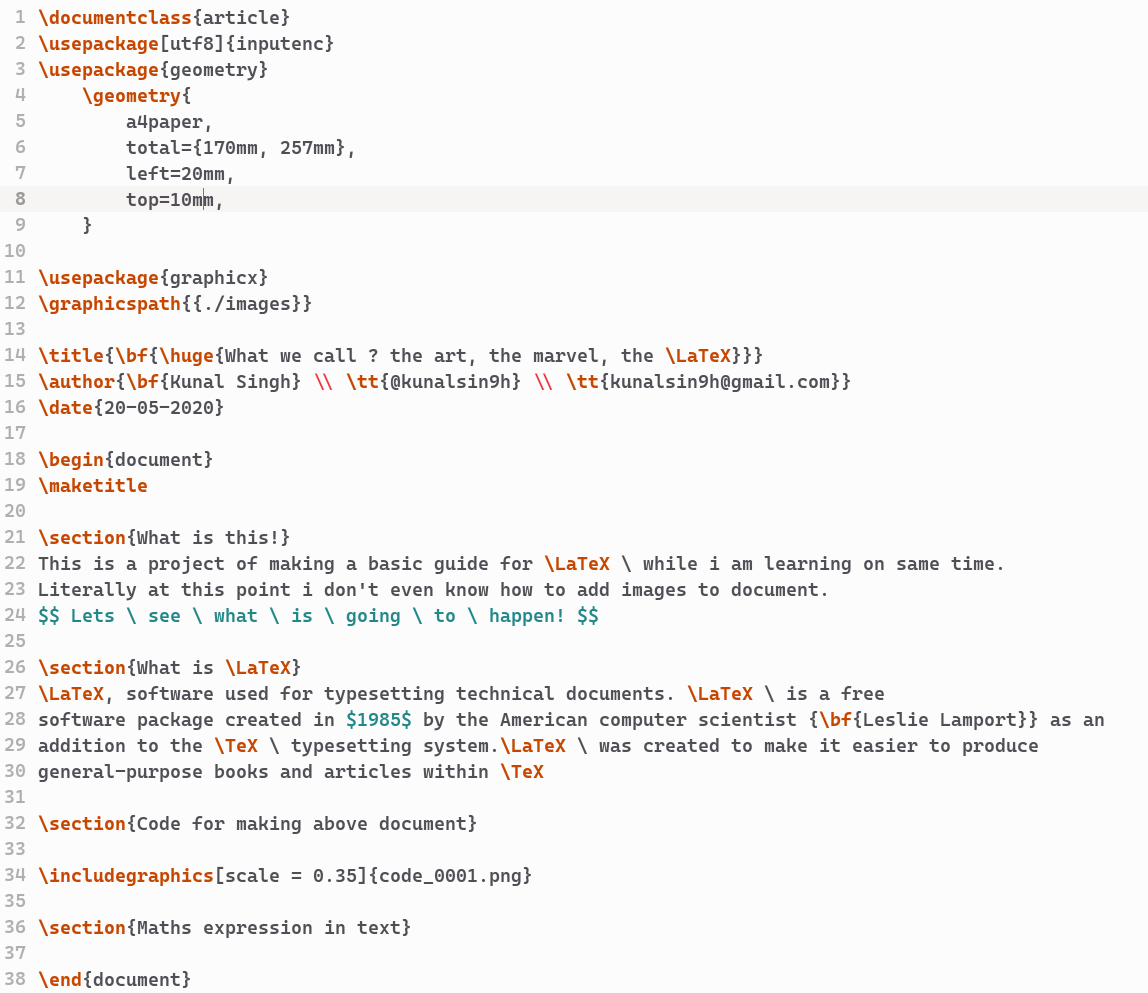
\includegraphics[scale = 0.35]{code_0001.png}

\section{Explaning Above code.}

\end{document}
